\documentclass[border=3mm,
               tikz,
               preview,
               qconvert
               ]{standalone}
\usepackage{pgfplots}

    \begin{document}
%---------------------------------------------------------------%
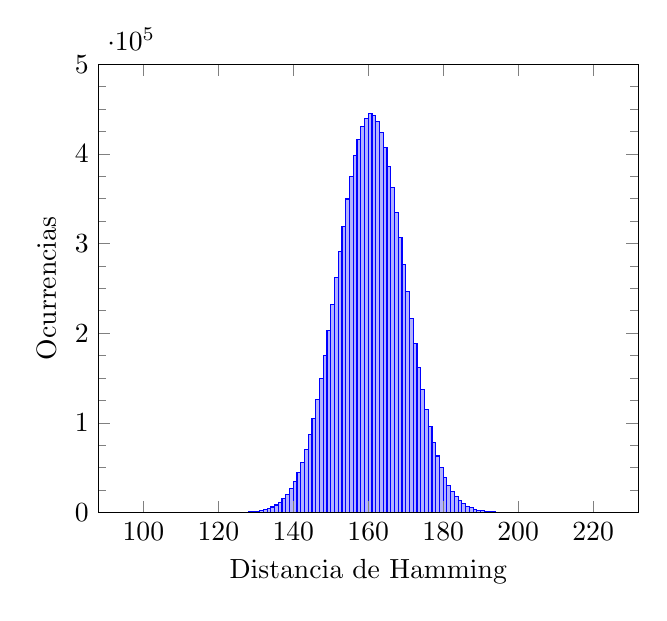
\begin{tikzpicture}
\begin{axis}[
    ymin=0, ymax=500000,
    minor y tick num = 3,
    area style,
    ylabel = {Ocurrencias},
    xlabel = {Distancia de Hamming},
    ]
\addplot+[ybar interval,mark=no] plot coordinates { 
(100,0)
(101,0)
(102,0)
(103,0)
(104,0)
(105,0)
(106,0)
(107,0)
(108,0)
(109,0)
(110,0)
(111,0)
(112,0)
(113,0)
(114,2)
(115,3)
(116,4)
(117,3)
(118,8)
(119,9)
(120,13)
(121,27)
(122,58)
(123,73)
(124,133)
(125,195)
(126,288)
(127,447)
(128,677)
(129,1006)
(130,1494)
(131,2231)
(132,3193)
(133,4334)
(134,6105)
(135,8366)
(136,11300)
(137,15390)
(138,20364)
(139,26656)
(140,34281)
(141,44594)
(142,55956)
(143,70175)
(144,86591)
(145,105090)
(146,125968)
(147,149111)
(148,175218)
(149,202730)
(150,231982)
(151,262301)
(152,291512)
(153,319478)
(154,349662)
(155,374701)
(156,397916)
(157,415878)
(158,430114)
(159,439852)
(160,444961)
(161,443279)
(162,436238)
(163,423918)
(164,407207)
(165,386250)
(166,362491)
(167,335045)
(168,306481)
(169,276700)
(170,246978)
(171,216865)
(172,188687)
(173,161610)
(174,137508)
(175,115267)
(176,95723)
(177,78177)
(178,63024)
(179,50037)
(180,39181)
(181,30607)
(182,23442)
(183,17878)
(184,13318)
(185,9770)
(186,7095)
(187,5126)
(188,3558)
(189,2564)
(190,1825)
(191,1278)
(192,857)
(193,563)
(194,354)
(195,219)
(196,171)
(197,114)
(198,68)
(199,32)
(200,18)
(201,11)
(202,9)
(203,1)
(204,3)
(205,0)
(206,2)
(207,1)
(208,0)
(209,0)
(210,0)
(211,0)
(212,1)
(213,0)
(214,0)
(215,0)
(216,0)
(217,0)
(218,0)
(219,0)
(220,0)
    
 };
\end{axis}
\end{tikzpicture}
    \end{document}
